\documentclass[11pt,a4paper]{article}

\usepackage[margin=2.5cm]{geometry}
\usepackage{hyperref}
\usepackage{amsmath,amssymb}
\usepackage{parskip}
\usepackage{microtype}
\usepackage{titlesec}
\usepackage{abstract}
\usepackage{booktabs}
\usepackage{array}
\usepackage{tikz}
\usetikzlibrary{positioning,arrows.meta,backgrounds,fit}
\usepackage{graphicx}

\titleformat{\section}{\large\bfseries}{\thesection}{0.6em}{}
\titleformat{\subsection}{\normalsize\bfseries}{\thesubsection}{0.6em}{}

\title{\textbf{Branched Multi-Turn GRPO for Code-Policy Generation on a Single GPU}}
\author{}
\date{}

\begin{document}
\maketitle

\begin{abstract}
\noindent
Multi-turn RL for code-generating agents fails mainly at credit
assignment: a single trajectory-level advantage cannot tell whether
success came from good planning or good final execution. This paper
targets that gap in code-policy generation, where an LLM writes a
Python \texttt{policy} and receives only the final scenario reward as
supervision. The central idea is to treat chat turns as macro-steps:
branch rollouts at turn boundaries, estimate per-turn Monte Carlo
values, and assign turn-specific advantages (VinePPO-style, but at
turn granularity). To make this practical on a single 24\,GB GPU, loss
computation is decomposed across turns using the additivity of the
token-summed clipped surrogate, reducing peak LM-head activation memory
from $\sum_n T_n$ to $\max_n T_n$ without changing the accumulated
gradient. The resulting method is a compact synthesis of existing RL
ingredients (GRPO, VinePPO, hierarchical credit assignment), specialized
for multi-turn code-policy training under tight compute constraints.
Experiments instantiate the method at $N{=}2$ with $G_1{=}G_2{=}4$; the
extension to $N{>}2$ is straightforward.
\end{abstract}

\section{Introduction}

Reinforcement-learning fine-tuning of LLMs has converged on a small
set of recipes: PPO with a learned critic, GRPO and its DAPO/CISPO
variants which replace the critic with a group-relative Monte Carlo
baseline, and process-supervision pipelines that train an auxiliary
reward model. Most of this work targets single-turn reasoning, where
the trajectory is a prompt followed by one completion and the reward
is observed at the end. Extending these recipes to multi-turn
agentic settings exposes a credit-assignment problem: a single
trajectory-level advantage broadcast to every model token cannot
distinguish a strong first-turn strategy followed by poor execution
from the converse.

This problem is studied in the setting of \emph{code-policy
generation}: the LLM emits a Python \texttt{def policy(state)} body
that is executed across environment scenarios in an isolated
subprocess. The artifact is code; the LLM is removed from the
inner control loop at deployment. The protocol uses $N$ chat turns:
intermediate turns may draft a candidate \texttt{policy} (whose
scenario reward is returned as a tool message) or run a \texttt{main}
scratchpad (stdout returned as feedback), and the final turn commits the
scored \texttt{policy}. The scheme is instantiated and evaluated at
$N{=}2$.

The training scheme has two components. First, trajectory-level credit
assignment is replaced with a per-turn branched rollout
and per-turn MC value estimates --- the macro-step analog of
VinePPO's intra-completion branching, with hierarchical baselines
conditioned on the prefix at each turn boundary. Second, to make the
resulting trajectories trainable on a 24\,GB L4, the
additivity of the token-summed clipped surrogate over disjoint token
subsets sharing the same global normalizer is exploited to
run forward and backward passes for each turn independently. Peak LM-head
saved-activation memory drops from
$O(B\cdot \sum_n T_n\cdot |V|)$ to
$O(B\cdot \max_n T_n\cdot |V|)$ without changing the accumulated
gradient: the parameter gradients summed across the per-turn passes
equal the single-pass gradient exactly. The trade-off is compute ---
each later pass recomputes the prefix of earlier turns ---
not gradient quality.

This combination is a straightforward specialization of standard
mechanisms rather than a new algorithm. The contribution is a clean
assembly that fits on a single small GPU, plus a loss decomposition
that makes that budget feasible.

\section{Related work}

\paragraph{Critic-free LLM RL.} GRPO~\cite{shao2024deepseekmath} and
its token-summed variants (DAPO~\cite{yu2025dapo}, CISPO) replace
PPO's learned critic with a group-relative MC baseline. The
token-summed form is used because its additivity over token subsets
makes the per-turn loss decomposition exact.

\paragraph{Branching for credit assignment.} The closest existing
method is VinePPO~\cite{kazemnejad2024vineppo}, which estimates
$\widehat V(s_t)$ at chosen intra-completion states via on-policy MC
re-branching and uses it as a per-token baseline. The same
mechanism is used, but branching occurs only at \emph{turn boundaries} of a chat
trajectory and broadcast the resulting advantage as a constant within
each turn --- group-relative within a turn, VinePPO-like across
turns.

\paragraph{Hierarchical multi-turn agents.}
ArCHer~\cite{zhou2024archer} adopts the same macro-step decomposition
(per-turn value, per-token policy update) but learns the per-turn
value with a critic. Here it is estimated by MC over $G_2$ continuations,
trading variance for the cost of fitting a value head.
ReBN~\cite{liu2025gem} replaces GAE with batch-normalized MC returns;
the hierarchical mean used here can be viewed as ReBN partitioned by
turn-1 prefix. RAGEN's StarPO~\cite{wang2025ragen} is the canonical
flat-baseline critic-free MC scheme for multi-turn LLM RL; setting
$G_2=1$ collapses our scheme to it.

\paragraph{$G_1\times G_2$ tree rollouts.} The same tree shape appears
in process-reward-model training pipelines such as
Math-Shepherd~\cite{wang2024mathshepherd} and
OmegaPRM~\cite{luo2024omegaprm}, where the per-prefix MC mean labels
intermediate steps for a learned reward model. The tree is used as a
policy-gradient baseline rather than as a labelling oracle.

\paragraph{Code policies.} Voyager~\cite{wang2024voyager} and
FunSearch~\cite{romera-paredes2024funsearch} also produce executable
code as the artifact, but rely on frozen-LLM prompting plus
skill-library accumulation or evolutionary mutation respectively. The LLM
is adapted with gradient-based RL of LoRA weights and a
scratchpad turn between prompt and committed code.

\section{Method}

\subsection{Setup}
\label{sec:setup}

The agent is a language model $\pi_\theta$ over chat-template
trajectories. The base is \texttt{Qwen2.5-Coder-3B-Instruct} with
frozen weights $W$; $\theta$ parameterizes a LoRA adapter
$W' = W + AB^\top$. A task $\mathcal{T}$ specifies environment source
code, $S$ scenarios $\{\sigma_i\}$ that vary the seed and hidden
parameters, and a per-scenario reward. The scoring oracle runs a
candidate policy body in a sandboxed subprocess against each scenario
and returns
\(
  R(\text{code};\mathcal{T}) = \sum_i r_i(\text{code};\sigma_i).
\)
Validation failures, errors, and timeouts on $\sigma_i$ score the
\emph{error floor} $r_i = -200$, calibrated below any
running-but-failing trajectory --- otherwise errored rollouts ($r=0$)
outrank running-but-poor rollouts and the gradient rewards crashing.

\subsection{Chat-template protocol}
\label{sec:protocol}

Each turn the model emits one fenced code block tagged \texttt{policy}
or \texttt{main}. \texttt{policy} defines \texttt{def policy(state)},
which the tool executes across all scenarios and reports the summed
reward as a user-role message. \texttt{main} is arbitrary scratchpad
code with no environment access; the tool returns truncated stdout.
The final turn must be \texttt{policy}; \texttt{main} or untagged
final turns are floored. Malformed intermediate turns are likewise
floored and surfaced as a textual rejection. A length-$N$ trajectory
is
\(
  \tau = (s,\, y^{(1)},\, m^{(1)},\, \dots,\, y^{(N-1)},\, m^{(N-1)},\, y^{(N)}),
\)
with completions $y^{(n)}$ alternating with tool messages $m^{(n)}$,
and $R(\tau) = R(\text{code in }y^{(N)})$ the only scalar reward.
The remainder of the paper specializes to $N{=}2$: a single
intermediate turn (draft policy or scratchpad) followed by a committed
\texttt{policy}. Generalizing the rollout, advantages, and loss
decomposition below to $N{>}2$ is straightforward (see
\S\ref{sec:limitations}).

\subsection{Token-summed clipped surrogate}

For trajectory $b$ at position $t$, with importance ratio
$\rho^b_t = \pi_\theta / q$ and per-token advantage $A^b_t$,
\begin{equation}
\mathcal{L}(\theta) =
 -\frac{1}{N_{\text{tok}}}\sum_{b,t}
   \mathbf{1}\{\text{model token}\}\cdot
   \min\!\big(\rho^b_t A^b_t,\,\mathrm{clip}(\rho^b_t,\,1-\epsilon_{\text{lo}},\,1+\epsilon_{\text{hi}}) A^b_t\big),
\label{eq:loss}
\end{equation}
with $N_{\text{tok}}$ the count of model tokens in the global batch.\footnote{This
matches the DAPO and CISPO recipes; per-row averaging variants
(original GRPO, BNPO, Dr.GRPO) divide by per-row token counts.}
\eqref{eq:loss} is \emph{additive over disjoint token subsets}: for
any partition of model-token positions, the loss equals the sum of
partial losses computed with the same $N_{\text{tok}}$. This is the
property the per-turn decomposition (\S\ref{sec:per-turn-decomp}) exploits.

\subsection{Branched rollout}

For each prompt $s$, sample $G_1$ turn-1 variants in one
\texttt{model.generate} call:
$y^{(1)}_i \sim q(\cdot\mid s)$, $i=1,\dots,G_1$. For each $y^{(1)}_i$
execute the tool to obtain $m_i$, then sample $G_2$ continuations
$y^{(2)}_{i,j} \sim q(\cdot\mid s, y^{(1)}_i, m_i)$ in one call. Score
each leaf to obtain $\{R_{i,j}\}$. Generate-call cost per prompt is
$1+G_1$, versus $2G_1 G_2$ for an unbranched rollout with the same
number of leaves.

\subsection{Per-turn MC value estimates and advantages}

Two empirical values, both pure averages over the tree:
\begin{equation}
  \widehat V_0 = \frac{1}{G_1 G_2}\sum_{i,j} R_{i,j},
  \qquad
  \widehat V_1^{(i)} = \frac{1}{G_2}\sum_{j} R_{i,j}.
\end{equation}
$\widehat V_0$ estimates the initial-state value;
$\widehat V_1^{(i)}$ the value after committing to turn-1 variant
$y^{(1)}_i$. Per-turn advantages, broadcast to every token of the
corresponding turn:
\begin{align}
  A^{(1)}_{i}      &= \widehat V_1^{(i)} - \widehat V_0
    & \text{(over $y^{(1)}_i$)}, \label{eq:adv1}\\
  A^{(2)}_{i,j}    &= R_{i,j} - \widehat V_1^{(i)}
    & \text{(over $y^{(2)}_{i,j}$).} \label{eq:adv2}
\end{align}
The turn-2 advantage uses the conditional mean given the turn-1
prefix rather than the global per-prompt mean: a poor turn-2 sample
drawn from a strong turn-1 is recognized as poor instead of
inheriting its prefix's above-average outcome. Tool-message tokens
are masked via \texttt{tool\_mask}; their advantage is zero.
Figure~\ref{fig:credit-assignment} contrasts this scheme with the
two closest critic-free / per-turn-credit baselines for multi-turn
LLM RL.

\begin{figure}[t]
\centering
\resizebox{\linewidth}{!}{%
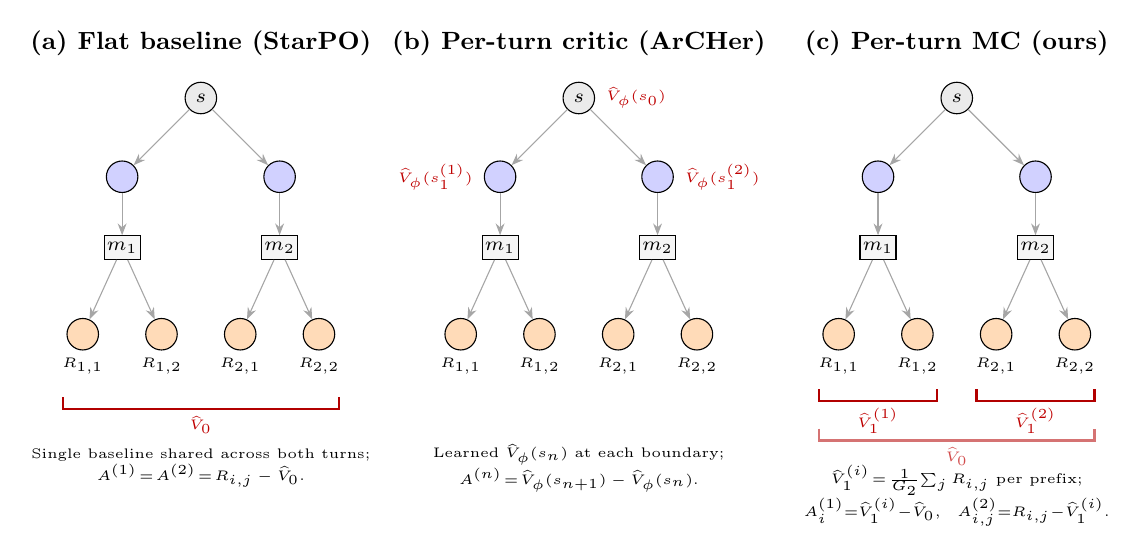
\begin{tikzpicture}[
  >={Stealth[length=1.5mm]},
  every node/.style={font=\scriptsize, inner sep=1pt},
  prompt/.style={circle, draw, fill=black!8,  minimum size=4mm},
  t1/.style    ={circle, draw, fill=blue!18,  minimum size=4mm},
  t2/.style    ={circle, draw, fill=orange!28, minimum size=4mm},
  tool/.style  ={rectangle, draw, fill=black!4,
                 minimum width=4mm, minimum height=3mm},
  rew/.style   ={font=\tiny},
  bln/.style   ={font=\tiny, color=red!75!black, anchor=west},
  arr/.style   ={->, draw=gray!70},
  panel/.style ={font=\small\bfseries},
]

%%% Shared geometry for all three panels (vertical layout):
%%%   prompt   y = 5.0   (centered)
%%%   turn-1   y = 4.0
%%%   tool     y = 3.1
%%%   turn-2   y = 2.0
%%%   reward   y ≈ 1.55  (just below leaves)
%%%   bracket  y ∈ [0.8, 1.25]
%%%   caption  y ≈ -0.2
%%% x-axis: 0.2 / 1.2 / 2.2 / 3.2 for the four leaves; panel width ≈ 3.4

%%% (a) Flat baseline — StarPO / Arm D
\begin{scope}
  \node[panel] at (1.7, 5.7) {(a) Flat baseline (StarPO)};
  \node[prompt] (sa) at (1.7, 5.0) {$s$};
  \node[t1] (y1a1) at (0.7, 4.0) {};
  \node[t1] (y1a2) at (2.7, 4.0) {};
  \node[tool] (ma1) at (0.7, 3.1) {$m_1$};
  \node[tool] (ma2) at (2.7, 3.1) {$m_2$};
  \node[t2] (y2a11) at (0.2, 2.0) {};
  \node[t2] (y2a12) at (1.2, 2.0) {};
  \node[t2] (y2a21) at (2.2, 2.0) {};
  \node[t2] (y2a22) at (3.2, 2.0) {};
  \node[rew, below=0.5mm of y2a11] {$R_{1,1}$};
  \node[rew, below=0.5mm of y2a12] {$R_{1,2}$};
  \node[rew, below=0.5mm of y2a21] {$R_{2,1}$};
  \node[rew, below=0.5mm of y2a22] {$R_{2,2}$};
  \draw[arr] (sa) -- (y1a1);  \draw[arr] (sa) -- (y1a2);
  \draw[arr] (y1a1) -- (ma1); \draw[arr] (y1a2) -- (ma2);
  \draw[arr] (ma1) -- (y2a11); \draw[arr] (ma1) -- (y2a12);
  \draw[arr] (ma2) -- (y2a21); \draw[arr] (ma2) -- (y2a22);
  % Single V_0 bracket spanning all four leaves, below rewards
  \draw[red!70!black, thick] (-0.05, 1.20) -- (-0.05, 1.05)
    -- (3.45, 1.05) -- (3.45, 1.20);
  \node[bln, anchor=north] at (1.7, 1.00) {$\widehat V_0$};
  \node[align=center, font=\tiny] at (1.7, 0.30)
    {Single baseline shared across both turns;\\
     $A^{(1)}\!=\!A^{(2)}\!=\!R_{i,j}-\widehat V_0$.};
\end{scope}

%%% (b) Per-turn learned critic — ArCHer
\begin{scope}[xshift=4.8cm]
  \node[panel] at (1.7, 5.7) {(b) Per-turn critic (ArCHer)};
  \node[prompt] (sb) at (1.7, 5.0) {$s$};
  \node[t1] (y1b1) at (0.7, 4.0) {};
  \node[t1] (y1b2) at (2.7, 4.0) {};
  \node[tool] (mb1) at (0.7, 3.1) {$m_1$};
  \node[tool] (mb2) at (2.7, 3.1) {$m_2$};
  \node[t2] (y2b11) at (0.2, 2.0) {};
  \node[t2] (y2b12) at (1.2, 2.0) {};
  \node[t2] (y2b21) at (2.2, 2.0) {};
  \node[t2] (y2b22) at (3.2, 2.0) {};
  \node[rew, below=0.5mm of y2b11] {$R_{1,1}$};
  \node[rew, below=0.5mm of y2b12] {$R_{1,2}$};
  \node[rew, below=0.5mm of y2b21] {$R_{2,1}$};
  \node[rew, below=0.5mm of y2b22] {$R_{2,2}$};
  \draw[arr] (sb) -- (y1b1);  \draw[arr] (sb) -- (y1b2);
  \draw[arr] (y1b1) -- (mb1); \draw[arr] (y1b2) -- (mb2);
  \draw[arr] (mb1) -- (y2b11); \draw[arr] (mb1) -- (y2b12);
  \draw[arr] (mb2) -- (y2b21); \draw[arr] (mb2) -- (y2b22);
  % Per-state learned-critic values, side-annotated on the boundary nodes.
  % s_0 to the right of s, s_1^{(i)} between turn-1 variant and tool message.
  \node[bln] at (sb.east) [anchor=west, xshift=1mm] {$\widehat V_\phi(s_0)$};
  \node[bln] at (y1b1.west) [anchor=east, xshift=-1mm] {$\widehat V_\phi(s_1^{(1)})$};
  \node[bln] at (y1b2.east) [anchor=west, xshift=1mm] {$\widehat V_\phi(s_1^{(2)})$};
  \node[align=center, font=\tiny] at (1.7, 0.30)
    {Learned $\widehat V_\phi(s_n)$ at each boundary;\\
     $A^{(n)}\!=\!\widehat V_\phi(s_{n+1})-\widehat V_\phi(s_n)$.};
\end{scope}

%%% (c) Per-turn MC — Ours
\begin{scope}[xshift=9.6cm]
  \node[panel] at (1.7, 5.7) {(c) Per-turn MC (ours)};
  \node[prompt] (sc) at (1.7, 5.0) {$s$};
  \node[t1] (y1c1) at (0.7, 4.0) {};
  \node[t1] (y1c2) at (2.7, 4.0) {};
  \node[tool] (mc1) at (0.7, 3.1) {$m_1$};
  \node[tool] (mc2) at (2.7, 3.1) {$m_2$};
  \node[t2] (y2c11) at (0.2, 2.0) {};
  \node[t2] (y2c12) at (1.2, 2.0) {};
  \node[t2] (y2c21) at (2.2, 2.0) {};
  \node[t2] (y2c22) at (3.2, 2.0) {};
  \node[rew, below=0.5mm of y2c11] {$R_{1,1}$};
  \node[rew, below=0.5mm of y2c12] {$R_{1,2}$};
  \node[rew, below=0.5mm of y2c21] {$R_{2,1}$};
  \node[rew, below=0.5mm of y2c22] {$R_{2,2}$};
  \draw[arr] (sc) -- (y1c1);  \draw[arr] (sc) -- (y1c2);
  \draw[arr] (y1c1) -- (mc1); \draw[arr] (y1c2) -- (mc2);
  \draw[arr] (mc1) -- (y2c11); \draw[arr] (mc1) -- (y2c12);
  \draw[arr] (mc2) -- (y2c21); \draw[arr] (mc2) -- (y2c22);
  % Inner V_1^(i) brackets — one per turn-1 prefix, spans G_2 leaves of that prefix
  \draw[red!70!black, thick] (-0.05, 1.30) -- (-0.05, 1.15)
    -- (1.45, 1.15) -- (1.45, 1.30);
  \node[bln, anchor=north] at (0.7, 1.10) {$\widehat V_1^{(1)}$};
  \draw[red!70!black, thick] (1.95, 1.30) -- (1.95, 1.15)
    -- (3.45, 1.15) -- (3.45, 1.30);
  \node[bln, anchor=north] at (2.7, 1.10) {$\widehat V_1^{(2)}$};
  % Outer V_0 bracket — root mean over all four leaves, drawn beneath V_1 brackets
  \draw[red!70!black, thick, opacity=0.55] (-0.05, 0.80) -- (-0.05, 0.65)
    -- (3.45, 0.65) -- (3.45, 0.80);
  \node[bln, anchor=north, opacity=0.7] at (1.7, 0.60) {$\widehat V_0$};
  \node[align=center, font=\tiny] at (1.7, -0.05)
    {$\widehat V_1^{(i)}\!=\!\tfrac{1}{G_2}\!\sum_j R_{i,j}$ per prefix;\\
     $A^{(1)}_i {=} \widehat V_1^{(i)}{-}\widehat V_0,\ \
      A^{(2)}_{i,j} {=} R_{i,j}{-}\widehat V_1^{(i)}$.};
\end{scope}

\end{tikzpicture}%
}
\caption{Comparison of credit-assignment mechanisms on a 2-turn
branched rollout from prompt $s$ with $G_1{=}G_2{=}2$. All three
panels show the same rollout structure --- turn-1 fan-out
$\{y^{(1)}_i\}$, tool message $m_i$, turn-2 fan-out
$\{y^{(2)}_{i,j}\}$, leaf rewards $R_{i,j}$ --- and differ only in
how the per-token baseline is computed.
\textbf{(a) Flat baseline} (StarPO / RAGEN~\cite{wang2025ragen}, the
N=2 generalization of RLOO/GRPO~\cite{shao2024deepseekmath} from
Figure~2 of \cite{kazemnejad2024vineppo}): one mean $\widehat V_0$
over all $G_1 G_2$ leaves, broadcast to every model token of both
turns. A poor turn-2 from a strong turn-1 inherits its prefix's
above-average outcome.
\textbf{(b) Per-turn critic} (ArCHer~\cite{zhou2024archer}): a
learned value head $\widehat V_\phi(s_n)$ provides per-state
baselines at each turn boundary, with the moving-target bias issues
typical of bootstrapped value learning.
\textbf{(c) Per-turn MC} (ours, Arm~F): the conditional mean
$\widehat V_1^{(i)} = \tfrac{1}{G_2}\sum_j R_{i,j}$ over the $G_2$
continuations of turn-1 variant $i$ baselines that variant's turn-1
tokens; $\widehat V_0$ baselines the root. Turn-2 tokens are scored
against their own prefix's $\widehat V_1^{(i)}$, not the global
mean. Group-relative within a turn, VinePPO-like across turns ---
i.e., VinePPO's intra-completion MC re-branching
\cite{kazemnejad2024vineppo}, applied at turn boundaries.}
\label{fig:credit-assignment}
\end{figure}

\subsection{Per-turn loss decomposition}
\label{sec:per-turn-decomp}

The token-summed clipped surrogate \eqref{eq:loss} factors over any
partition of the model-token positions into disjoint subsets that
share the same global normalizer $N_{\text{tok}}$. Letting
$\mathcal{I}_n$ index the model tokens of turn $n$,
\begin{equation}
  \mathcal{L} = \sum_{n=1}^{N} \mathcal{L}_{\mathcal{I}_n},
  \qquad N_{\text{tok}} = \sum_{n=1}^{N} |\mathcal{I}_n|.
\label{eq:additive}
\end{equation}
Per-row averaged variants (original GRPO, BNPO, Dr.GRPO) do
\emph{not} factor this way: each row carries its own denominator,
so the partial sums do not combine into the single-row loss. The
token-summed form is what makes the decomposition exact.

\eqref{eq:additive} is exploited to compute $\mathcal{L}$ in $N$
forward/backward passes rather than one. Pass $n$ forwards
$[s \,|\, y^{(1)} \,|\, m^{(1)} \,|\, \dots \,|\, y^{(n)}]$,
computes $\mathcal{L}_{\mathcal{I}_n}$, backwards, and frees. By
\eqref{eq:additive} the parameter gradients accumulated across the
$N$ passes equal the single-pass gradient exactly.

\paragraph{Why this saves memory.} The dominant activation cost is
the LM head's logit tensor, with $|V| \approx 152{,}000$ for our base
model. The HF \texttt{logits\_to\_keep} API materializes logits only
at the positions where they are needed for the loss
(Appendix~\ref{app:memory}); at training time those are the model-
emitted token positions. In a single forward+backward over the full
trajectory, the autograd graph holds the saved-for-backward LM-head
tensors at all $\sum_n T_n$ model-token positions across all turns
simultaneously, until backward completes. By computing each turn's
loss in a separate forward+backward, only one turn's
saved-for-backward tensors are held at peak ($T_n^{\max}$ positions), and
the graph is freed before the next turn begins. The decomposition is
gradient accumulation at the turn level within a trajectory: same
accumulated gradient by \eqref{eq:additive}, lower peak activation
memory by a factor of roughly $N$ when turns are equal-length.
Appendix~\ref{app:memory} has concrete numbers for $N{=}2$; at our
settings the saving over a careful single-pass implementation is
roughly $2\times$.

\paragraph{Restrictions.} The decomposition's exactness has one
\emph{conceptual} requirement and two \emph{implementation}
requirements. Conceptual: the token-summed normalizer of
\eqref{eq:loss} --- per-row averaged variants do not factor across
token-position partitions, as discussed above. Implementation:
$\beta=0$ (a KL term to $\pi_{\text{ref}}$ would require per-segment
slicing of reference log-probabilities) and
\texttt{num\_iterations}$=1$ (so cached
\texttt{old\_per\_token\_logps} need no re-segmenting). The two
implementation requirements can be lifted with extra bookkeeping at
no theoretical cost (\S\ref{sec:limitations}).

\section{Experimental setup}

\paragraph{Why this environment.} Standard RL benchmarks are a poor
fit for evaluating LoRA fine-tuning of a code-policy LLM. CartPole
and similar two-line tasks are solved at iteration 0 by the base
model, giving a flat learning curve. LunarLander, Pendulum,
MountainCar, and other named environments are heavily represented in
pretraining corpora, so any improvement is confounded with recall
rather than learning. The task therefore requires source code that the model has to
\emph{read} rather than recognize, with non-trivial dynamics and a
clear ceiling above the base-model prior. The puck-on-tilted-plane
environment below was designed to fit those constraints: a small
custom dynamics file, hidden per-scenario parameters that defeat
look-up strategies, and a tight thrust envelope that rules out the
naive one-line policy.

A second motivation, specific to the multi-turn protocol, is partial
observability. The hidden tilt, drag, and thrust limit are not part
of the state vector but they fully determine which control gains
work; a policy that writes itself blind to those parameters is
limited to whatever conservative gains succeed across the whole
prior. The protocol gives the model an explicit affordance for
\emph{system-identification probes} in the rehearsal turn: a
\texttt{main} scratchpad that applies short thrust patterns,
inspects the resulting velocities via stdout, and uses the readings
to size the committed policy's gains. Whether the trained model
actually exploits this affordance --- rather than collapsing to a
robust prior --- is itself an empirical question the protocol makes
testable.

\paragraph{Environment.} A 2D puck-on-tilted-plane controller. The
puck moves in $[-6, 6]^2$ under a constant hidden tilt $(t_x, t_y)$
and linear drag $\mu$; the policy receives
$\{p_x,p_y,v_x,v_y,g_x,g_y\}$ and must drive the puck to a goal
within 120 steps. Hidden parameters --- tilt, drag, thrust limit
$a_{\max}$, initial velocity --- vary per scenario and are not in the
state. The thrust envelope is set to
$a_{\max} = \|\text{tilt}\|_2 \times 1.05 + \epsilon$ so a naive
straight-at-goal policy fails because it cannot cancel tilt drift.
Per-step reward is $-\Delta t\cdot\text{dist}(p, g)$ with a $+50$
bonus on reaching the goal; errored episodes hit the floor of
\S\ref{sec:setup}.

\paragraph{Baseline gap.} Two hand-written policies fix the headroom:
naive aim ($\approx 26\%$ goal rate over 200 seeds) and
PD-with-tilt-feedforward ($\approx 73\%$). The gap is the room
LoRA fine-tuning has to exploit. The analogous baseline gap on the
slosh-tank environment (used for the experimental arms in
\S\ref{sec:eval}) is established by a $\kappa$ sweep of nominal-PD
vs.\ oracle-PD success rates in Appendix~\ref{app:slosh-sweep}.

\paragraph{Model and compute.} \texttt{Qwen2.5-Coder-3B-Instruct},
LoRA rank $r=16$ on attention and MLP projections, on a single
24\,GB L4 GPU. bf16 weights, gradient checkpointing on. The setup uses
$G_1 = G_2 = 4$ (16 leaves per prompt) and a per-turn token cap of
$400$.

\paragraph{Training.} The token-summed clipped surrogate
\eqref{eq:loss} with $\epsilon_{\text{lo}}=0.2$, asymmetric upper
clip, $\beta=0$, and the per-turn advantages of
\eqref{eq:adv1}--\eqref{eq:adv2}. No reference KL, no critic, no
GAE, no context truncation across turns.

\paragraph{Diagnostics.} Logged diagnostics include $\widehat V_0$ and the
between-variant standard deviation of $\widehat V_1$, the
within-variant standard deviation, and their ratio (the
\emph{signal ratio}); the per-turn advantage standard deviations;
the fraction of trajectories at the error floor; and the count of
\texttt{generate} calls per prompt (expected $1 + G_1$). The signal
ratio guides allocation between $G_1$ and $G_2$ at fixed budget:
$>1$ means turn-1 variation dominates and a larger $G_1$ helps; $<1$
means within-variant noise dominates and a larger $G_2$ helps.

\section{Evaluating the per-turn credit assignment}
\label{sec:eval}

The per-turn loss decomposition (\S\ref{sec:per-turn-decomp}) is purely a
memory enabler --- it does not change the gradient. The substantive
claim that requires empirical support is the \emph{credit-assignment}
contribution: hierarchical per-turn advantages
\eqref{eq:adv1}--\eqref{eq:adv2} on a $G_1\times G_2$ tree do better
than a single trajectory-level advantage broadcast across both turns.
Table~\ref{tab:ablation} defines a six-arm ablation, ordered from
the weakest baseline to the proposed method. Adjacent rows isolate a
single axis where possible (E~vs.~D isolates the tree; F~vs.~E
isolates the per-turn baseline). The frozen-to-trained jump (B~vs.~C)
and the single-to-multi-turn jump (C~vs.~D) each change two axes and
are interpreted accordingly.

\begin{table}[h]
\centering
\small
\begin{tabular}{@{}lp{3.2cm}p{4.3cm}p{4.0cm}@{}}
\toprule
Arm & Rollout structure & Advantage & What it isolates over the previous arm \\
\midrule
A --- Frozen, one-shot & $N{=}1$ inference, no training & --- & Base model's prior on the code-policy interface \\
B --- Frozen, multi-turn prompted & $N{=}2$ inference, no training & --- & Does the two-turn protocol help at inference time? (Voyager-/FunSearch-style frozen-LLM use) \\
C --- Single-turn GRPO & $G$ flat $N{=}1$ rollouts, trained & Standard GRPO advantage & Does RL fine-tuning help at all? \\
D --- Flat StarPO & $G$ independent $N{=}2$ trajectories, trained & $A(\tau) = R(\tau) - \bar R$, broadcast to all tokens & Does multi-turn training help over single-turn? (RAGEN-style) \\
E --- Branched, flat & $G_1{\times}G_2$ tree, trained & $A_{i,j} = R_{i,j} - \bar R$ on all tokens & Does the tree alone help (more leaves per generate call), independent of credit? \\
F --- Branched, hierarchical (ours) & $G_1{\times}G_2$ tree, trained & $A^{(1)}_i = \widehat V_1^{(i)} - \widehat V_0$ on $y^{(1)}_i$; $A^{(2)}_{i,j} = R_{i,j} - \widehat V_1^{(i)}$ on $y^{(2)}_{i,j}$ & The per-turn baseline contribution \\
\bottomrule
\end{tabular}
\caption{Ablation arms, ordered from weakest baseline (top) to ours
(bottom). Trained arms (C--F) match leaf count $G = G_1 G_2 = 16$ so
they see the same number of scored trajectories per step. D uses
$2G$ \texttt{generate} calls per prompt; F uses $1+G_1$. Report both
equal-rollouts and equal-wall-clock comparisons. Frozen arms (A, B)
use the same Qwen2.5-Coder-3B-Instruct base with no gradient updates,
and serve as training-free references analogous to Voyager- or
FunSearch-style frozen-LLM uses of the code-policy interface.}
\label{tab:ablation}
\end{table}

\paragraph{Primary metric.} Held-out goal rate on a stress
distribution (more extreme tilts/drag than train) at the best
checkpoint, reported as median and IQR over $\geq 3$ seeds per arm,
plotted against gradient steps and against wall-clock. Statistical
test: paired Wilcoxon over per-seed best-checkpoint goal rates;
report effect size, not just $p$. The minimum convincing comparison
is F $>$ D at matched leaves.

\paragraph{Diagnostic checks.}
Two further measurements sharpen the mechanism story.
\begin{enumerate}
  \item \emph{Turn-1 quality curve.} Track the mean reward of turn-1
        \texttt{policy} drafts (when turn-1 is in policy mode) as a
        function of training step. Under D the trajectory-level
        advantage projects onto turn-1 only through the global mean;
        under F, $A^{(1)}_i$ provides a direct gradient signal on
        turn-1 quality. F should show a steeper turn-1 reward rise
        than D.
  \item \emph{Signal-ratio conditioning.} The training loop already
        logs the per-prompt signal ratio
        $\widehat\sigma(\widehat V_1^{(i)})/\overline{\widehat\sigma(R_{i,\cdot})}$.
        Bucket prompts by their iteration-0 signal ratio. Ratio
        $>1$ means turn-1 choice dominates the variance and per-turn
        credit should help; ratio $<1$ means within-variant noise
        dominates and per-turn credit should not. F's advantage over
        D should grow with the bucket's signal ratio. If it does not,
        the mechanism is not doing what theory predicts and the
        headline claim weakens.
\end{enumerate}

\paragraph{Arm A: frozen one-shot baseline (preliminary).}
Table~\ref{tab:arm_a} reports the first completed arm.
Qwen2.5-Coder-3B-Instruct (no LoRA, $N{=}1$, temperature 0.8) achieves
\textbf{0\% success} at all three gain values $\kappa \in \{0.65, 0.80, 1.00\}$
over 20 sampled policies $\times$ 50 seeds each.
The mean reward $\approx -112$ is well below both the blind PD ($-10$ to $+112$
depending on $\kappa$) and the oracle ($+111$), a gap of $\approx\!223$ points.
Even the single best generated policy scores $-12.1$ at every $\kappa$,
confirming the base model cannot write a working controller zero-shot.
Two failure modes account for the result: $\approx$40\% of policies crash at
runtime (hallucinated state keys; penalised at $-200$), and the rest produce
control-theoretically wrong code (reversed-sign bang-bang, pendulum dynamics
mis-applied as a control law).
The flat reward across all three $\kappa$ values confirms the model has no
awareness of the hidden gain.
This large gap to both reference curves establishes that RL fine-tuning has
a clear training signal, validating the benchmark difficulty.

\begin{table}[h]
\centering
\small
\begin{tabular}{@{}ccccc@{}}
\toprule
$\kappa$ & Qwen 1-shot (mean) & Qwen 1-shot (max) & Blind PD & Oracle PD \\
\midrule
0.65 & $-112.0$ & $-12.1$ & $-9.6$  & $+111.2$ \\
0.80 & $-111.9$ & $-12.1$ & $+45.9$ & $+111.4$ \\
1.00 & $-111.9$ & $-12.1$ & $+111.5$ & $+111.5$ \\
\bottomrule
\end{tabular}
\caption{Arm A: frozen one-shot Qwen2.5-Coder-3B-Instruct vs.\ reference
policies on the slosh-tank task ($\kappa \in \{0.65, 0.80, 1.00\}$,
20 policy samples, 50 seeds each, $\kappa$ fixed per episode).
Mean reward averages over all samples; max is the best mean achieved by any
single generated policy.
Crashed policies scored at $-200$ (matching the GRPO training signal).
Oracle scales PD gains by $1/\kappa$; blind uses nominal gains.}
\label{tab:arm_a}
\end{table}

\paragraph{Arm B: frozen two-turn baseline (preliminary).}
Table~\ref{tab:arm_b} reports the second completed arm: the same model
in the two-turn probe-then-adapt prompt ($N{=}2$, temperature 0.8, 20
sampled policies $\times$ 50 seeds per $\kappa$). Arm~B was run after
adopting \texttt{Qwen3-4B-Instruct-2507} as the study's base model; for
direct comparability, the 1-turn run was repeated on the same base and
is included as the third column of Table~\ref{tab:arm_b}.
Table~\ref{tab:arm_a}'s Qwen2.5-Coder-3B numbers remain as the original
Arm~A record.

\emph{The format gate fires, the value transfer does not.}
60/60 samples open turn 1 with \texttt{\# MODE: main} and call
\texttt{env.reset()} --- vs.\ 27\% \texttt{main}-mode usage on the
earlier 3B baseline; 21/60 also step the env at least once with a known
commanded acceleration. Yet \textbf{0/60 samples compute a $\kappa$
estimate} from the probe data: the arithmetic that would turn the
printed $\Delta v$ into a gain estimate ---
$\kappa \approx \Delta v / (a_{\text{cmd}}\,\Delta t)$ at
$\theta\!\approx\!\omega\!\approx\!0$ on a single step --- is never
written, even when all of $a_{\text{cmd}}$, $\Delta v$, and $\Delta t$
are on screen. The protocol's intent appears in 60/60 turn-1 comments
(``probing the environment to gain insights about the hidden actuator
gain $\kappa$''); the corresponding code appears zero times.

\emph{Mean reward improves modestly; success rate does not.}
The 2-turn per-sample median mean-reward exceeds the 1-turn median by
12--18 points at every $\kappa$ ($-57.7$ vs.\ $-76.3$ at $\kappa=0.65$;
$-74.2$ vs.\ $-86.8$ at $\kappa=0.80$; $-68.2$ vs.\ $-86.5$ at
$\kappa=1.00$), consistent with the model writing slightly better
controllers in turn~2 after seeing the state shape printed in turn~1 ---
a weak format-side effect, not information gathering. Success rate
stays $\leq 0.7\%$ across all $\kappa$, driven by a single
$\kappa=0.65$ sample whose Pattern-D (reset-only) probe transferred no
information and whose turn-2 body is a clean four-state PD controller
earning $+5.7$ mean reward and 14\% per-seed success rate --- the
first positive frozen-baseline reward on the slosh task, and an
instance of \emph{control reasoning} improving rather than
probe-then-adapt operating.

The probe-then-adapt protocol is therefore \emph{nominal but not
operative}: every sample passes the format gate, the prompt's
instruction to probe is followed, but the value the protocol is
supposed to deliver --- a $\kappa$ estimate that conditions the turn-2
controller --- never materialises. The headline gap RL fine-tuning has
to close is exactly to make $\kappa$-estimation arithmetic appear in
turn-1 probe code and be \emph{read} by the turn-2 policy. The signal
the trainer needs is supplied by the $G_2$ branched continuations of
\S\ref{sec:per-turn-decomp}: a turn-1 probe that contains the
information turn-2 needs should produce, on average, higher-reward
$G_2$ leaves, and the per-turn baseline $\widehat V_1^{(i)}$ of
Figure~\ref{fig:credit-assignment}~(c) is what propagates that signal
back to turn-1 tokens.

\begin{table}[h]
\centering
\small
\begin{tabular}{@{}ccccc@{}}
\toprule
$\kappa$ & Naive PD & Oracle PD & Qwen3-4B 1-turn & Qwen3-4B 2-turn \\
\midrule
0.65 & $0\%$   & $100\%$ & $0\%$   & $\mathbf{0.7\%}^{\dagger}$ \\
0.80 & $46\%$  & $100\%$ & $0.5\%$ & $0\%$ \\
1.00 & $100\%$ & $100\%$ & $0.7\%$ & $0\%$ \\
\bottomrule
\end{tabular}
\caption{Arms~A and~B on \texttt{Qwen3-4B-Instruct-2507} vs.\ reference
controllers on the slosh-tank task. Success rate is the fraction of 50
episodes simultaneously meeting all four settling conditions
($|x{-}g|, |v|, |\theta|, |\omega|$), averaged over 20 generated
policies. Naive uses nominal PD gains; oracle scales gains by $1/\kappa$.
$^{\dagger}$The $\kappa=0.65$ Arm~B aggregate is driven by a single
outlier sample with 14\% per-seed success; the per-sample distribution
is otherwise within sampling noise of the 1-turn column at $n{=}20$
(median rewards $-57.7$ vs.\ $-76.3$). The best Arm~B sample is the
first positive frozen-baseline mean reward observed on this task.}
\label{tab:arm_b}
\end{table}

\paragraph{Failure modes to declare upfront.} If F $\not>$ D under
matched leaves, the hierarchical baseline does not improve results in this
domain and the contribution reduces to ``branching amortizes generate
calls'' (E vs D). If F $\approx$ E but both beat D, the gain is from
the tree structure, not from the per-turn baseline. If the trained
arms (C--F) do not clearly beat the frozen arms (A, B), RL
fine-tuning adds little over the base model's prior under
this protocol, and the work is better framed as
prompt-engineering rather than training. If B $>$ A, the multi-turn
protocol itself provides training-free gains, and that gap should be
part of the headline result.

\section{Limitations and future work}
\label{sec:limitations}

The scheme is instantiated and evaluated at $N{=}2$. Extension
to $N{>}2$ is straightforward: each $\widehat V_n^{(\cdot)}$ becomes the
conditional MC mean over the subtree below it, and the two-pass loss
decomposition becomes an $N$-pass decomposition by the same
additivity argument (\eqref{eq:additive}). Neither is conceptually
new, but both add bookkeeping and are not implemented or
benchmarked here. This work assumes
deterministic environments given the seed --- under stochastic
dynamics the leaf rewards become noisier estimates of state values
and $G_2$ would have to grow accordingly. The $\beta=0$,
\texttt{num\_iterations}$=1$ restrictions are implementation
choices that the same decomposition argument can lift with extra
per-segment slicing of reference log-probabilities and cached
sampling log-probabilities.

\paragraph{Token subsampling.} A direct extension is to backprop
through only a fraction $\alpha \in (0, 1]$ of the model-emitted
tokens per turn rather than all of them. Because each turn's
advantage $A^{(n)}$ is a single scalar broadcast across all of that
turn's tokens, every token contributes a sample of the same
population gradient: subsampling is a sample-variance loss, not the
information loss it would be in supervised fine-tuning where each
token has a distinct target. The token-summed normalizer of
\eqref{eq:loss} keeps the resulting estimator unbiased for any
$\alpha$ when $N_{\text{tok}}$ is updated to count only the kept
positions; per-row averaged variants would be biased by uneven
drops across trajectories, an additional reason the token-summed
form is the right baseline. The memory benefit compounds with the
per-turn decomposition: peak LM-head saved-activation memory drops
from $\max_n T_n$ to $\alpha \max_n T_n$, on top of the
$\sum_n T_n \to \max_n T_n$ saving of \S\ref{sec:per-turn-decomp}.
Two variants suggest themselves as ablation arms.
\emph{Uniform per-turn:} drop a fixed fraction within every turn,
to test whether the variance increase hurts convergence at all
given the broadcast-advantage redundancy.
\emph{Asymmetric per-turn:} keep all of the committed turn $y^{(N)}$
but only $\alpha$ of the rehearsal turns $y^{(<N)}$, to test
whether explicitly biasing learning toward the artifact helps over
treating all turns symmetrically. The asymmetric variant has no
single-turn analog. These experiments were not run here.

\section{Conclusion}

A critic-free, on-policy multi-turn RL scheme for
code-policy generation that combines branched rollouts with per-turn
MC value estimates and a per-turn loss decomposition. The algorithmic
ingredients are individually standard; the assembly is small enough
to train on a single 24\,GB GPU, and the per-turn decomposition ---
which the token-summed normalizer makes exact --- is what keeps it
that way as the number of turns grows.

\appendix

\section{Memory accounting and the trailing-window LM-head}
\label{app:memory}

This appendix walks through why a single forward over a multi-turn
trajectory is expensive and where the per-turn decomposition's
saving comes from. It is written for readers who are familiar with
policy-gradient RL but not necessarily with the internals of LLM
training. The argument turns on a single API constraint in HF
\texttt{transformers} which we make explicit here rather than in the
body.

\paragraph{The LLM as an autoregressive policy.} A causal LLM is a
stochastic policy whose action space at each step is the vocabulary
$\mathcal{V} = \{1, \dots, |V|\}$. Given a sequence of $T$ token IDs
as input, the model produces, at each position $t$, a logit vector
$\ell_t \in \mathbb{R}^{|V|}$; the next-token distribution is
$\mathrm{softmax}(\ell_t)$, and the log-prob of having emitted token
$a$ at position $t{+}1$ is $\log\mathrm{softmax}(\ell_t)_a$. To form
the policy-gradient surrogate \eqref{eq:loss} we need exactly these
log-probs at every position $t$ such that $t{+}1$ was a
\emph{model-emitted} token. Logits at other positions --- prompt
positions, and (in our multi-turn setting) tool-message positions
--- are not needed for the gradient and are wasted compute if we
materialize them.

\paragraph{Where the memory goes.} The model splits into two pieces
with very different memory profiles. We distinguish three buckets
because the asymmetry between them is what motivates the
decomposition: \emph{parameter weights}, \emph{per-position activations
saved for backward}, and \emph{per-position output of the LM head}.

\emph{Transformer body.} A stack of $L \approx 36$ blocks (attention
$+$ MLP), holding the bulk of the $3{\cdot}10^9$ parameters. Each
block produces per-position activations of width $O(d)$ with
$d \approx 2048$. Without optimization the body's saved activations
for backward are $O(L \cdot d)$ per position. We use gradient
checkpointing, which recomputes intermediate block activations during
backward instead of storing them, leaving only $O(d)$ per position
saved at checkpoint boundaries. So in our setup the body holds many
parameters but small per-position activations.

\emph{LM head.} A single linear layer of shape $(d, |V|)$:
${\sim}3{\cdot}10^8$ parameters --- modest --- but its per-position
\emph{output} is the full logit vector of width $|V| \approx
152{,}000$. The head sits at the end of the graph, so checkpointing
it would buy nothing (there is nothing upstream to recompute through
the loss): its full $(B, T, |V|)$ output is held until backward, with
an equal-sized autograd buffer for the gradient.

\emph{The asymmetry.} Once gradient checkpointing is on, the body
keeps roughly $d \approx 2{,}000$ floats of activation per position,
while the LM head keeps roughly $|V| \approx 152{,}000$. The head's
per-position activation is ${\sim}75\times$ the body's, and unlike
the body it cannot be checkpointed away. Body parameter weights are
larger in absolute terms but they are loaded once and shared across
all positions in the batch; the head's $(B, T, |V|)$ output scales
with both batch size and trajectory length. At our trajectory
lengths the LM-head activation tensors are the term that pushes a
single-pass forward over budget, while parameters, optimizer state,
and gradient-checkpointed body activations are fixed costs that fit
under any of the regimes below. \emph{The decomposition therefore
saves peak LM-head activation memory specifically, not total GPU
memory in equal proportion} --- an important distinction when
reading Table~\ref{tab:memory}.

\paragraph{The \texttt{logits\_to\_keep} parameter.} Because most
positions' logits are not needed for the loss, HF
\texttt{transformers} lets you specify which ones to compute. The
forward call accepts an argument \texttt{logits\_to\_keep}
(historically \texttt{num\_logits\_to\_keep}) of type
\texttt{int} \emph{or} 1D \texttt{torch.Tensor}.\footnote{See e.g.\
the Qwen2 forward signature in HF \texttt{transformers}: the slice
is \texttt{slice(-K, None)} for an int and the tensor itself for a
1D \texttt{torch.Tensor}.} With an integer $K$, the LM head is
applied to the last $K$ hidden states, producing logits of shape
$(B, K, |V|)$. With a 1D tensor of indices, the head is applied at
exactly those positions in the sequence dimension. Either way, only
the selected positions' logits are materialized and held for
backward. The transformer body still runs over all $T$ positions
because causal self-attention chains every position to its prefix,
but the body is two orders of magnitude cheaper per position than
the LM head.

\paragraph{The constraint that actually matters.} The API can select
arbitrary subsets of positions, so the issue is not which positions
can be reached. The issue is autograd: a single forward+backward
holds the saved-for-backward LM-head tensors at \emph{all} selected
positions in memory simultaneously, until \texttt{loss.backward()}
returns. Peak LM-head activation memory therefore scales with the
total number of selected positions, regardless of whether they are
contiguous.

For multi-turn training the total is $\sum_n T_n$ --- every model-
emitted token across every turn. The per-turn decomposition
sidesteps this by doing one forward+backward per turn and freeing
the graph between, so peak LM-head memory scales with $\max_n T_n$
instead. The trick is identical in spirit to gradient accumulation
across micro-batches: the same accumulated gradient is computed, but
peak activation memory is shrunk by serializing what would otherwise
be parallel.

\paragraph{Three regimes.} Concretely, with $T_1 = T_2 = 400$, prompt
$\approx 500$, tool message $\approx 50$, batch $B = 16$ leaves per
prompt, $|V| = 152{,}000$, and 4-byte logits (the autograd
intermediate is held in fp32 for the cross-entropy reduction even
when weights are bf16):

\begin{table}[h]
\centering
\small
\begin{tabular}{@{}lll@{}}
\toprule
Regime & Positions through LM head & Logit tensor \\
\midrule
(a) Single pass, no \texttt{logits\_to\_keep} & $T_{\text{full}} = 1350$ & $\approx 13.1$\,GB \\
(b) Single pass, tensor \texttt{logits\_to\_keep} (model tokens) & $\sum_n T_n = 800$ & $\approx 7.8$\,GB \\
(c) Two passes (ours), int \texttt{logits\_to\_keep}$=\max_n T_n$ per pass & $400$ per pass, freed between & $\approx 3.9$\,GB \\
\bottomrule
\end{tabular}
\caption{LM-head logit tensor size under each regime, plus an
equal-sized autograd buffer for the backward pass (not shown).
Regime~(a) is the truly naive single forward. Regime~(b) is what a
careful single-forward implementation does, using the 1D-tensor form
of \texttt{logits\_to\_keep} to select exactly the model-token
positions across all turns. Regime~(c) is the per-turn decomposition
of \S\ref{sec:per-turn-decomp}, which holds at most one turn's
LM-head saved-for-backward tensors at peak.}
\label{tab:memory}
\end{table}

The relevant comparison for this setting is (b) vs.\ (c) --- a roughly
$2\times$ saving for $N{=}2$, scaling to $\sim N\times$ as the number
of equal-length turns grows. Regime~(a) is shown for completeness
but is not what a careful implementation actually does.

\paragraph{Arithmetic, not measured.} The numbers in
Table~\ref{tab:memory} are arithmetic from the LM-head output tensor
shape $(B, K, |V|)$ at 4 bytes per element; peak end-to-end GPU memory
under the three regimes has not yet been measured. End-to-end memory
also includes parameter weights and gradients, optimizer state,
gradient-checkpointed body activations, KV-cache (during rollout, not
training), masks, and allocator overhead. The decomposition's
expected effect is on the LM-head activation term specifically, and a
benchmark comparing measured peak GPU memory under (b) and (c) at the
same batch size, trajectory length, and model would provide a direct
empirical complement to the arithmetic above. That benchmark has not
yet been run.

\paragraph{What the per-turn decomposition is and isn't.} It is not a
new memory optimization over \texttt{logits\_to\_keep}; it is gradient
accumulation at the turn level within a trajectory. The HF API
already supports specifying any subset of positions for which to
compute logits, so all three regimes above use the same primitive ---
the difference is whether saved-for-backward tensors are held
simultaneously through one backward call or sequentially through $N$
backward calls. The non-trivial observation is that the gradients
accumulated across per-turn passes equal the single-pass gradient
\emph{exactly} (eq.\ \ref{eq:additive}), and that this exactness
depends on the token-summed normalizer of \eqref{eq:loss}. Per-row-
averaged GRPO variants would have to fall back to a single forward
(regime b) or accept a normalizer approximation.

\paragraph{Implementation note.} Pass~1 forwards $[s \,|\, y^{(1)}]$
as a self-contained sequence with $\texttt{logits\_to\_keep} = T_1$.
Pass~2 forwards the full trajectory but packs
$[s \,|\, y^{(1)} \,|\, m]$ into the prompt slot of HF's training
interface and $y^{(2)}$ alone into the completion slot, so
$\texttt{logits\_to\_keep} = T_2$ behaves as expected.

\section{Slosh-tank environment: design and dimensionless parameter analysis}
\label{app:slosh}

This appendix introduces the slosh-tank environment and derives the
dimensionless groups that govern whether a hidden unknown can actually
be exploited by a probe-and-adapt two-turn policy. The analysis applies
to any custom mechanics environment designed for this protocol; the
puck env of \S\ref{sec:setup} is the prior case.

\subsection*{Environment}

A one-dimensional cart carries liquid modelled as one damped pendulum mode
(slosh angle $\theta$, angular velocity $\omega$). The policy commands
horizontal acceleration, clipped to $[-1,\,1]$\,m/s$^2$. Observed state:
$\{t,\, x,\, v,\, \theta,\, \omega,\, g,\, \text{steps\_left}\}$.
Five hidden per-scenario parameters are absent from the state:

\smallskip
\begin{center}
\small
\begin{tabular}{@{}lll@{}}
\toprule
Parameter & Symbol & Role \\
\midrule
Actuator gain  & $\kappa$ & Scales commanded acceleration before actuation \\
Action delay   & $D$      & Steps before a command reaches the actuator \\
Deadband       & $b$      & Commands $|a|<b$ produce no output \\
Slosh length   & $L$      & Pendulum length; sets slosh natural frequency \\
Damping        & $c$      & Linear damping on the slosh mode \\
\bottomrule
\end{tabular}
\end{center}
\smallskip

Dynamics (semi-implicit Euler, $\Delta t = 0.06$\,s):
\begin{align}
a_{\mathrm{true}} &= \kappa \cdot \mathrm{deadband}(a_{\mathrm{cmd}[t-D]}), \notag \\
v &\mathrel{+}= \Delta t \cdot a_{\mathrm{true}}, \quad x \mathrel{+}= \Delta t \cdot v, \\
\dot\omega &= -\tfrac{g}{L}\,\theta - c\,\omega - a_{\mathrm{true}}, \quad \dot\theta = \omega. \notag
\end{align}

Success requires all four conditions simultaneously:
$|x - g| < \epsilon_x$, $|v| < \epsilon_v$, $|\theta| < \epsilon_\theta$,
$|\omega| < \epsilon_\omega$. This prevents policies that ram the cart to
position without settling the liquid.

\subsection*{Physical parameters and their dimensions}

Setting aside the integration step, success thresholds, and reward weights,
eight parameters govern the dynamics (fundamental dimensions: $\mathsf{L}$,
$\mathsf{T}$; angles are dimensionless):

\begin{center}
\small
\begin{tabular}{@{}lllll@{}}
\toprule
Parameter & Symbol & Value & Dimension \\
\midrule
Gravitational acceleration & $g$              & 9.81\,m\,s$^{-2}$        & $\mathsf{L\,T}^{-2}$ \\
Max commanded acceleration & $a_{\max}$        & 1.00\,m\,s$^{-2}$        & $\mathsf{L\,T}^{-2}$ \\
Cart$\to$slosh coupling    & $\eta$           & 1.00\,m$^{-1}$           & $\mathsf{L}^{-1}$    \\
Slosh pendulum length      & $L$              & 0.70\,m                  & $\mathsf{L}$         \\
Slosh damping rate         & $c$              & 0.06\,s$^{-1}$           & $\mathsf{T}^{-1}$    \\
Goal distance              & $D_g$            & ${\sim}1.8$\,m           & $\mathsf{L}$         \\
Episode time               & $T_{\mathrm{ep}}$ & 6.3\,s                  & $\mathsf{T}$         \\
Actuator gain (hidden)     & $\kappa$         & $\{0.65,\,0.80,\,1.00\}$ & $1$                  \\
\bottomrule
\end{tabular}
\end{center}

\smallskip\noindent
The coupling $\eta$ enters the slosh dynamics as $\dot\omega = \cdots -
\eta\,a_{\mathrm{true}}$; for $\dot\omega\in[\mathsf{T}^{-2}]$ and
$a_{\mathrm{true}}\in[\mathsf{L\,T}^{-2}]$ one requires $[\eta]=\mathsf{L}^{-1}$,
equivalent to an inverse coupling-arm length. At $\eta=1.0$\,m$^{-1}$ the
effective arm is 1\,m, independent of the pendulum length $L$.

\subsection*{Buckingham $\pi$ theorem}

With 7 dimensional parameters and 2 fundamental dimensions, the theorem
yields $7-2=5$ independent dimensionless groups, plus $\kappa$ directly.
Choose $a_{\max}$ [$\mathsf{L\,T}^{-2}$] and $D_g$ [$\mathsf{L}$] as
repeating variables, defining time scale $\sqrt{D_g/a_{\max}}$.
Applying the theorem to each remaining parameter:

\begin{center}
\small
\begin{tabular}{@{}llll@{}}
\toprule
Group & Expression & Value & Non-repeating parameter \\
\midrule
$\pi_1$ & $g / a_{\max}$                         & $9.81$ & $g$ \\
$\pi_2$ & $\eta\,D_g$                             & $1.80$ & $\eta$ \\
$\pi_3$ & $L / D_g$                               & $0.39$ & $L$ \\
$\pi_4$ & $c\,\sqrt{D_g / a_{\max}}$              & $0.080$ & $c$ \\
$\pi_5$ & $T_{\mathrm{ep}}\,\sqrt{a_{\max}/D_g}$ & $4.70$ & $T_{\mathrm{ep}}$ \\
$\pi_6=\kappa$ & $\kappa$                         & $\{0.65,0.80,1.00\}$ & (already dimensionless) \\
\bottomrule
\end{tabular}
\end{center}

Products and ratios of $\pi$ groups are equally valid. The physically
interpretable recombinations are:
\begin{align}
T_{\mathrm{tr}} &= 2\sqrt{D_g/a_{\max}} = 2.68\;\text{s}
  \quad\text{(minimum bang-bang transit)},
  \label{eq:slosh_Ttr}\\
\tau &= \tfrac{1}{2}\pi_5 = \frac{T_{\mathrm{ep}}}{T_{\mathrm{tr}}} = 2.35
  \quad\text{(episode slack)},
  \label{eq:slosh_tau}\\
N_s &= \frac{1}{\pi}\sqrt{\frac{\pi_1}{\pi_3}} = \frac{T_{\mathrm{tr}}}{T_s}
  = 1.60\;\text{(slosh cycles per transit)},
  \label{eq:slosh_Ns}\\
\zeta &= \frac{\pi_4}{2\sqrt{\pi_1/\pi_3}} = \frac{c}{2\omega_n}
  = 0.008\;\text{(damping ratio)},
  \label{eq:slosh_zeta}\\
\theta_{\mathrm{ss}} &= \frac{\pi_2\,\pi_3}{\pi_1}
  = \frac{\eta\,a_{\max}\,L}{g}
  = 0.071\;\text{rad}\quad\text{(equilibrium slosh at full thrust).}
  \label{eq:slosh_thetass}
\end{align}
$\theta_{\mathrm{ss}}$ involves no tolerance parameter yet matches
$\epsilon_\theta = 0.07$\,rad to within rounding --- a constraint that
falls directly from the dynamics. Any final approach at full commanded
acceleration will fail the slosh condition; near-goal corrections must be
gentle.

\subsection*{When each unknown actually matters}

\paragraph{Actuator gain ($\kappa$).}
A gain-unaware controller plans transit assuming $\kappa=1$; at true gain
$\kappa<1$ the actual transit takes $1/\sqrt{\kappa}$ times longer by
\eqref{eq:slosh_Ttr}. Transit timeout occurs when
\begin{equation}
\tau < \frac{1}{\sqrt{\kappa_{\min}}}.
\label{eq:gain_cond}
\end{equation}
At $\kappa_{\min}=0.65$ and $\tau=2.35$, this condition is not met ($2.35 >
1.24$): the controller still has slack for transit. The empirically observed
gap arises through the settling phase: at $\kappa < 1$ the actuator delivers
only $\kappa$-attenuated corrections in the near-goal regime, slowing
convergence in position, velocity, and slosh simultaneously. Confirmed at
$N_{\rm steps}=105$: a blind nominal PD achieves $0\%$ success at
$\kappa=0.65$ while an oracle (gains divided by $\kappa$) achieves $100\%$,
with a clean transition from $0\%$ to $100\%$ blind success between
$\kappa=0.75$ and $\kappa=0.90$.

\paragraph{Action delay ($D$).}
Delay adds phase to the closed-loop response. High-gain feedback becomes
marginally stable around $\delta \approx 0.3$--$0.5$ for typical position
gains. Even when feedback oscillates, the controller converges given
sufficient time. For delay to mandate a qualitatively different strategy
(trajectory planning with anticipatory braking rather than reactive
feedback), the episode must be short enough that slow oscillatory
convergence exceeds the time budget. At $\tau=2.35$ this condition is not
met for $D \in \{0,\,2,\,4\}$; it is marginal at $D \in \{0,\,4,\,8\}$.

\paragraph{Slosh length ($L$) and damping ($c$).}
Fixed anti-slosh gains tuned for $L_0$ become suboptimal at other lengths.
The mismatch exceeds the success threshold $\epsilon_\theta$ only when
$\zeta$ is small enough that settling requires many cycles, and when $\tau$
is tight enough that there is no time to wait. At current $\zeta = 0.008$
and $\tau = 2.35$, the nominal gains $k_\theta = 1.30$, $k_\omega = 0.45$
succeed across moderate $L$ variation: the available slack absorbs the gain
mismatch. Tightening $\tau$ below $1.5$ is expected to expose the
slosh-length gap.

\subsection*{Confirmed V1 configuration}

The confirmed V1 varies \textbf{actuator gain only}, with all other
parameters fixed at nominal:

\begin{center}
\small
\begin{tabular}{@{}llll@{}}
\toprule
Parameter & Symbol & V1 value & Status \\
\midrule
Episode steps & $N_{\rm steps}$ & 105 ($\tau=2.35$) & Confirmed \\
Actuator gain & $\kappa$ & $\{0.65,\,0.80,\,1.00\}$ & Confirmed; clean gap \\
Action delay & $D$ & 0 steps & Fixed (V1) \\
Deadband & $b$ & 0 & Fixed (V1) \\
Slosh length & $L$ & 0.70\,m & Fixed (V1) \\
Damping & $c$ & 0.06\,s$^{-1}$ & Fixed (V1) \\
\bottomrule
\end{tabular}
\end{center}

Actuator gain is chosen as the first unknown because its effect is a smooth
rescaling of the settling bandwidth, directly interpretable from a
short probe: the ratio of observed to commanded velocity change in the
linear regime estimates $\kappa$. The blind/oracle gap is empirically
confirmed in \S\ref{app:slosh-sweep} at 200 seeds per $\kappa$ level
with $N_{\rm steps}=105$.

\subsection*{Empirical blind-vs-oracle gap ($\kappa$ sweep)}
\label{app:slosh-sweep}

The dimensionless analysis above predicts that the V1 unknown should
matter through settling rather than transit, i.e.\ that a blind
controller's success rate should rise smoothly with $\kappa$ as the
near-goal corrections deliver the intended magnitude, while an oracle
rescaling its commands by $1/\kappa$ should succeed across the entire
range. Table~\ref{tab:slosh-sweep} and Figure~\ref{fig:slosh-sweep}
confirm this empirically on 200 seeds per $\kappa$ level. The blind
controller transitions from $0\%$ at $\kappa=0.65$ to $100\%$ at
$\kappa=0.90$ in a clean S-curve, with $\geq\!50$\,pp blind-vs-oracle
separation across $\kappa\in\{0.65,\,0.80\}$ and $\geq\!20$\,pp
separation across $\kappa\in\{0.65,\,0.85\}$. This separation is the
empirical headroom the per-turn credit-assignment scheme of
\S\ref{sec:per-turn-decomp} has to exploit; it also fixes the V1
$\kappa$ set $\{0.65,\,0.80,\,1.00\}$ used throughout the experimental
arms as one stress, one transitional, and one nominal level.

\begin{table}[h]
\centering
\small
\begin{tabular}{@{}lll@{}}
\toprule
$\kappa$ & Blind PD success & Oracle PD success \\
\midrule
0.65 & $0\%$    & $100\%$ \\
0.70 & $0\%$    & $100\%$ \\
0.75 & $25.5\%$ & $100\%$ \\
0.80 & $50.5\%$ & $100\%$ \\
0.85 & $85\%$   & $100\%$ \\
0.90 & $100\%$  & $100\%$ \\
\bottomrule
\end{tabular}
\caption{Blind (nominal PD gains) vs.\ oracle (PD gains divided by
$\kappa$) success rate over 200 seeds at each $\kappa$ level.
$N_{\rm steps}=105$, goal $\in [1.4,\,2.2]$\,m, $L=0.70$\,m. The blind
S-curve traverses $0\to 100$\% across $\kappa\in[0.65,\,0.90]$ while
the oracle stays pinned at $100\%$, leaving a measurable gap that
RL fine-tuning has to close.}
\label{tab:slosh-sweep}
\end{table}

\begin{figure}[h]
\centering
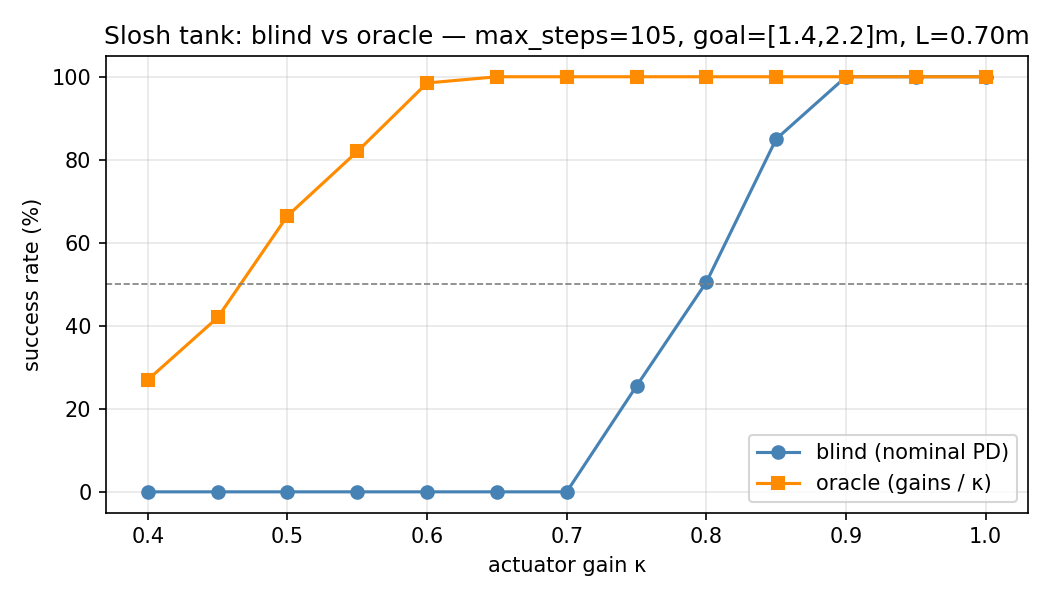
\includegraphics[width=0.78\textwidth]{slosh_gain_sweep.png}
\caption{Blind vs.\ oracle success rate as a function of actuator gain
$\kappa$ over 200 seeds per level (extends Table~\ref{tab:slosh-sweep}
to 13 $\kappa$ levels). The S-shape of the blind curve, together with
the oracle's flat $100\%$, is what makes the V1 setting a measurable
benchmark for probe-then-adapt: a controller that estimates $\kappa$
from a turn-1 probe and rescales its commands accordingly should track
the oracle curve rather than the blind curve. Generated by
\texttt{scripts/gain\_sweep.py}.}
\label{fig:slosh-sweep}
\end{figure}

\subsection*{Relation to the multi-turn protocol}

The two-turn protocol's value is testable only if there exists a real gap
between a policy written without probing and one written after observing
the first-turn trace. The dimensionless analysis above identifies the
parameter regime where this gap is non-trivial. Concretely, the required
baselines before any RL run are:
\begin{itemize}
  \item \emph{Blind nominal controller}: a fixed PD with standard anti-slosh
    gains, no first-turn probe. Sets the single-turn ceiling.
  \item \emph{Oracle-aware controller}: a controller that reads the hidden
    parameters directly and plans the optimal trajectory. Sets the two-turn
    ceiling.
  \item \emph{Probe-then-adapt controller}: a hand-written controller that
    runs the canonical pulse probe, estimates the unknown from the trace, and
    adapts its gains accordingly. The achievable probe-aware baseline.
\end{itemize}
The benchmark is useful for multi-turn RL only if
$\text{blind} < \text{probe-then-adapt} < \text{oracle}$ at the chosen
parameter setting.

\begin{thebibliography}{99}
\bibitem{shao2024deepseekmath} Z.~Shao et~al.
\emph{DeepSeekMath}. arXiv:2402.03300, 2024.
\bibitem{yu2025dapo} Q.~Yu et~al.
\emph{DAPO: An Open-Source LLM Reinforcement Learning System at
Scale}. arXiv:2503.14476, 2025.
\bibitem{kazemnejad2024vineppo} A.~Kazemnejad et~al.
\emph{VinePPO: Unlocking RL Potential For LLM Reasoning Through
Refined Credit Assignment}. arXiv:2410.01679, 2024.
\bibitem{wang2025ragen} Z.~Wang et~al. \emph{RAGEN: Training Agents
by Reinforcing Reasoning}. 2025.
\bibitem{liu2025gem} Z.~Liu et~al. \emph{GEM: Reinforcement Learning
for Generalist Models}. 2025.
\bibitem{zhou2024archer} Y.~Zhou et~al. \emph{ArCHer: Training
Language Model Agents via Hierarchical Multi-Turn RL}. ICML, 2024.
\bibitem{wang2024mathshepherd} P.~Wang et~al. \emph{Math-Shepherd}.
ACL, 2024.
\bibitem{luo2024omegaprm} L.~Luo et~al. \emph{Improve Mathematical
Reasoning in Language Models by Automated Process Supervision}.
arXiv:2406.06592, 2024.
\bibitem{wang2024voyager} G.~Wang et~al. \emph{Voyager}. TMLR, 2024.
\bibitem{romera-paredes2024funsearch} B.~Romera-Paredes et~al.
\emph{Mathematical discoveries from program search with large
language models}. Nature, 2024.
\end{thebibliography}

\end{document}
